\documentclass[paper=a4, fontsize=11pt]{scrartcl} % A4 paper and 11pt font size

\usepackage[T1]{fontenc} % Use 8-bit encoding that has 256 glyphs
\usepackage{fourier} % Use the Adobe Utopia font for the document - comment this line to return to the LaTeX default
\usepackage[english]{babel} % English language/hyphenation
\usepackage{amsmath,amsfonts,amsthm} % Math packages
%\usepackage{sectsty} % Allows customizing section commands
\usepackage{blindtext}
\usepackage[utf8]{inputenc}
\usepackage{sidecap}
\usepackage{graphicx}
\graphicspath{{images/}}
%\allsectionsfont{\left\normalfont\scshape} % Make all sections centered, the default font and small caps
\usepackage{fancyhdr} % Custom headers and footers
\pagestyle{fancyplain} % Makes all pages in the document conform to the custom headers and footers
\fancyhead{} % No page header - if you want one, create it in the same way as the footers below
\fancyfoot[L]{} % Empty left footer
\fancyfoot[C]{\thepage} % put page number in center footer
\fancyfoot[C]{} % Empty right footer
\renewcommand{\headrulewidth}{0pt} % Remove header underlines
\renewcommand{\footrulewidth}{0pt} % Remove footer underlines
\setlength{\headheight}{2pt} % Customize the height of the header

\numberwithin{equation}{section} % Number equations within sections (i.e. 1.1, 1.2, 2.1, 2.2 instead of 1, 2, 3, 4)
\numberwithin{figure}{section} % Number figures within sections (i.e. 1.1, 1.2, 2.1, 2.2 instead of 1, 2, 3, 4)
\numberwithin{table}{section} % Number tables within sections (i.e. 1.1, 1.2, 2.1, 2.2 instead of 1, 2, 3, 4)

\setlength\parindent{2pt} % Removes all indentation from paragraphs - comment this line for an assignment with lots of text

%----------------------------------------------------------------------------------------
%	TITLE SECTION
%----------------------------------------------------------------------------------------
\title{	
\normalfont \normalsize 
\textsc{EENG 517}\\ 
\huge Final Project \\ % The assignment title
}

\author{Dana Martin} % Your name

\date{\normalsize Due: End of Semester}

\begin{document}

\maketitle % Print the title

%----------------------------------------------------------------------------------------
%	Plant Description
%----------------------------------------------------------------------------------------
\begin{section}*{Plant Description}

	Task: Choose a system of interest and write down governing equations that will be used to tune a state-space controller.\\
	\newline
	Helicopters and wind turbines are intricately connected as many of the equations that govern one also, govern the other.  Both systems incorporate multi blade assemblies connected to a hub.  At the hub, actuators and sensors are used as correctors and feedback signals which optimize the performance of the system, making sure the plant stays and/or reaches a desired range of operation.  For this project, I will design a state-space feedback system for a 3 bladed single rotor helicopter with trailing edge blade mounted actuated flaps.  The model and equations of motion for this project are encouraged and aided by the work of Garcia et al \cite{Garcia}.\\
	
	A helicopter is a very complex and technologically advanced machine, and in its entirety, is out of the scope of this class so some simplifications must be made.  For this project, the allowable DOF will be the rotation around the hub, flap-wise bending and root flap pitch for a total of 3 DOF per blade totaling 9 DOF for a 3 bladed rotor.\\
	
	\begin{center}
	  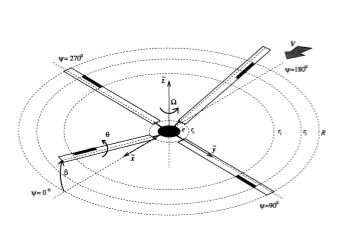
\includegraphics{RotorCoordinates}\\
	 {Stationary Rotor Coordinate System compliments of Garcia \cite{Garcia}}
	  \label{RotorCoordinates:RotorCoordinateSystem1}
	\end{center}
	
	The above figure shows a stationary Cartesian Coordinate System (x,y,z) attached at the hub, which will be used to calculate the rotor hub forces.  A second reference frame is needed in order to calculate the blade dynamics, which will be attached to the an individual blade and be allowed to rotate.    
	
		\begin{center}
		  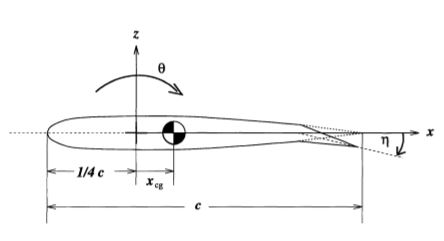
\includegraphics{RotorCoordinatesII}\\
		  {Rotating Rotor Coordinate System compliments of Garcia \cite{Garcia}}
		  \label{RotorCoordinatesII:RotorCoordinateSystem2}
		\end{center}
	
	
	\newpage
	\begin{thebibliography}{9}
	\bibitem{Garcia} 
	Garcia,J.C.(1994). \textit{Active Helicopter Rotor Control Using Blade-Mounted Actuators}.\\ Mechanical Engineering Department Massachusetts Institute of Technology.  
	\end{thebibliography}
	
\end{section}
\end{document}